\chapter{Implementation of the game}\label{ch:implementation}
\section{The Smart Contract}
	\begin{figure}[ht]
		\begin{center}
			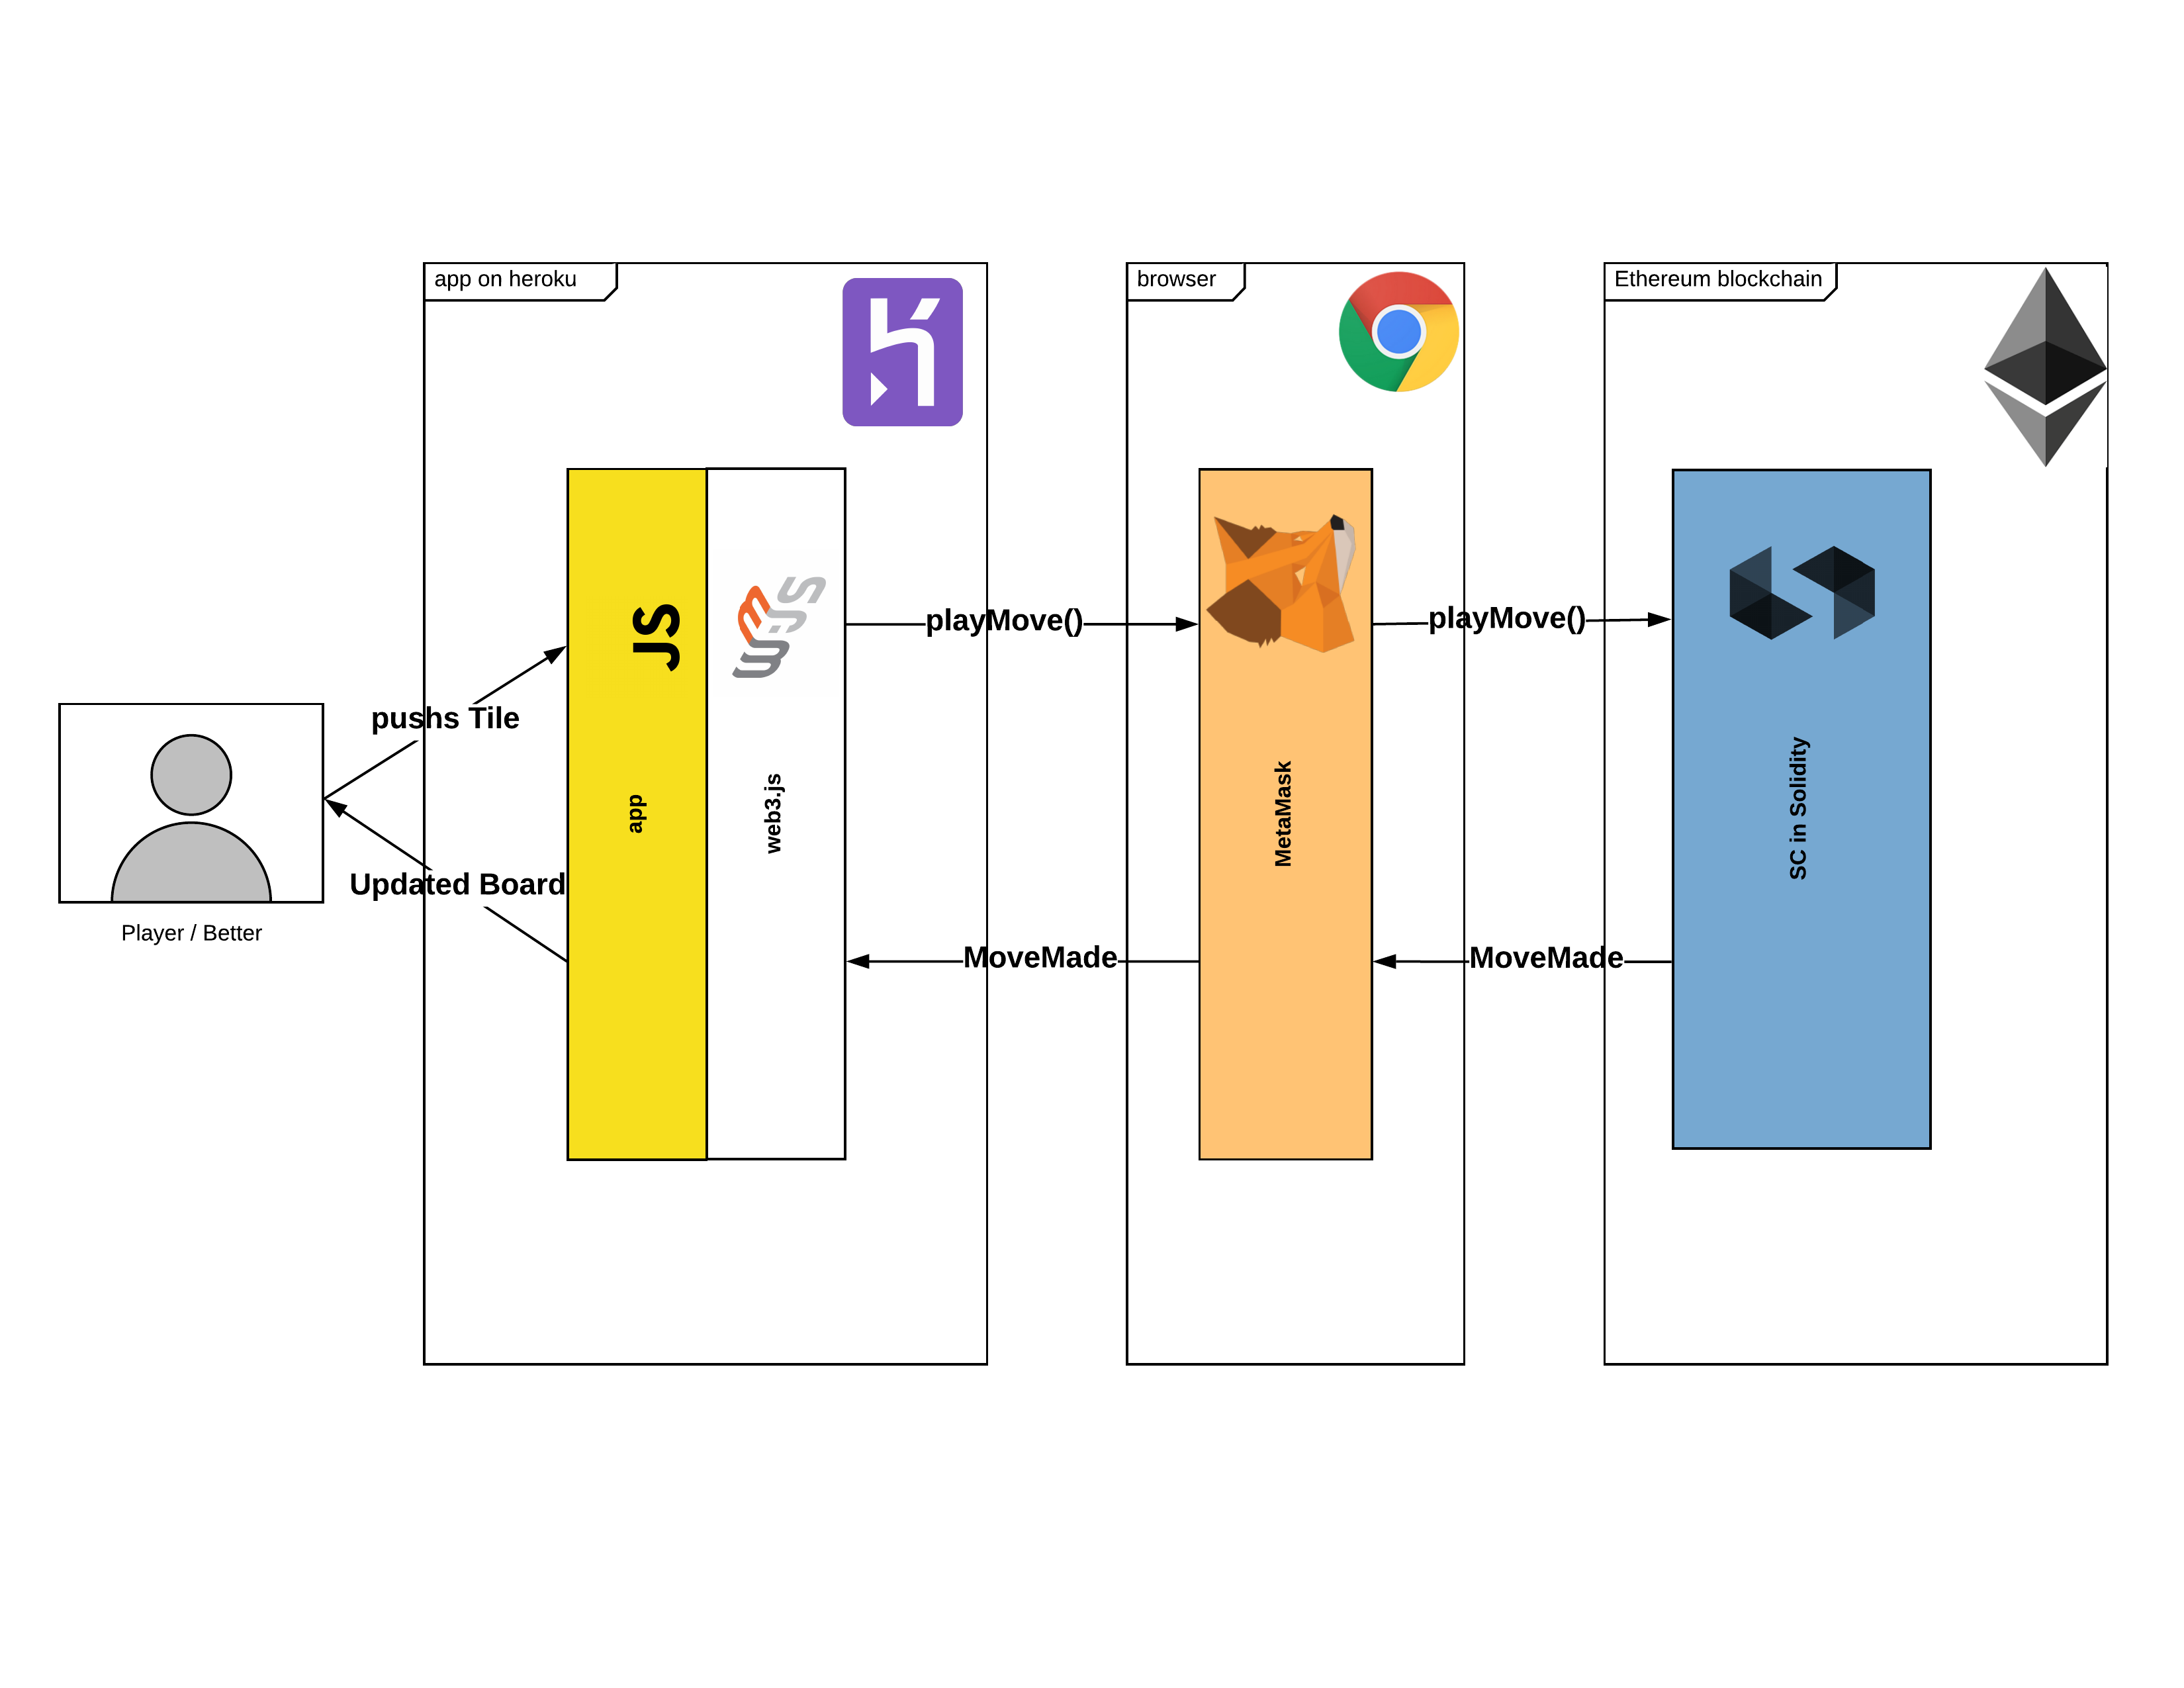
\includegraphics[scale=0.4]{res/project_structure}
		\end{center}
		\caption{Project Structure with Technologies}
		\label{fig:project_structure}
	\end{figure}	
Figure \ref{fig:project_structure} shows the project structure and the interaction between the different systems by the example of an Player choosing a tile on the board.
The web-application is running on the Heroku Platform\footnote{https://www.heroku.com/}. Through the browser and MetaMask a User can get verified by its Ethereum-account and pay the requested amount of gas in order to run functionalities on the Ethereum \ac{sc}. The \ac{sc} itself runs on an blockchain, which can be either a private or the Ropsten Testnet\footnote{https://ropsten.etherscan.io/}.\\
The \ac{sc} firstly checks if the move is valid. Secondly it looks for a winner and changes the game state if so. After that it returns a move confirmation to the user.

Three functions of the \ac{sc} we show here, as we consider them complex and interesting:\\




The class-diagram in Figure\ref{fig:sc_uml}  show a detail class diagram explaining the modelling and structure of our \ac{sc}
	\begin{figure}[ht]
		\begin{center}
			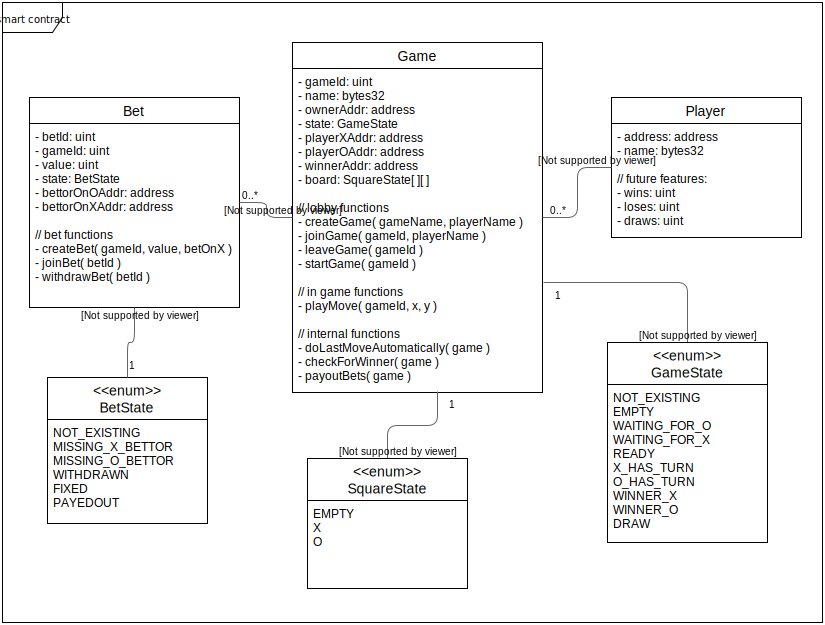
\includegraphics[scale=0.22]{res/sc_uml}
		\end{center}
		\caption{Class-Diagram of the \ac{sc}}
		\label{fig:sc_uml}
	\end{figure}
%logic and modell
